\documentclass{VUMIFPSbakalaurinis}
\usepackage{algorithmicx}
\usepackage{algorithm}
\usepackage{algpseudocode}
\usepackage{amsfonts}
\usepackage{amsmath}
\usepackage{bm}
%\renewcommand{\figurename}{Fig.}
%\addto\captionslithuanian{\renewcommand{\figurename}{Fig.}}
%\addto\captionsenglish{\renewcommand{\figurename}{Fig.}}
\usepackage{caption}
\usepackage{color}
\usepackage{float}
\usepackage{graphicx}
\usepackage{listings}
\usepackage{subfig}
\usepackage{wrapfig}
\usepackage{listings}
\usepackage{pgfplots}

\lstset {
  language=Scala,
  basicstyle=\footnotesize,
  numbers=left,
  stepnumber=1,
  showstringspaces=false,
  tabsize=1,
  breaklines=true,
  breakatwhitespace=false,
}

% Titulinio aprašas
\university{Vilniaus universitetas}
\faculty{Matematikos ir informatikos fakultetas}
\institute{Informatikos institutas}  % Užkomentavus šią eilutę - institutas neįtraukiamas į titulinį
\department{Programų sistemų bakalauro studijų programa}
\papertype{Bakalauro baigiamasis darbas}
\title{Translation Unit Granularization}
\titleineng{Kompiliatoriaus transliuojamo vieneto smulkinimas}
\author{Andrius Bentkus}
% \secondauthor{Vardonis Pavardonis}   % Pridėti antrą autorių
\supervisor{asist. dr. Vytautas Valaitis}
\reviewer{doc. dr. Vardauskas Pavardauskas}
\date{Vilnius – \the\year}

% Nustatymai
% \setmainfont{Palemonas}   % Pakeisti teksto šriftą į Palemonas (turi būti įdiegtas sistemoje)
\bibliography{bibliografija}

\begin{document}
\maketitle

%% Padėkų skyrius
% \sectionnonumnocontent{}
% \vspace{7cm}
% \begin{center}
%     Padėkos asmenims ir/ar organizacijoms
% \end{center}

\addtocounter{page}{1}

\sectionnonumnocontent{Summary}
This thesis presents an approach on how to speed up recompilation in a day to day programming scenario, benchmarks the performance improvements with various inputs and compares the gathered performance metrics to an already existing compiler.

Classic compilers treat a source file as an atomic translation unit in their compilation pipeline, the proposed approach tries to leverage the structure of modern programming languages to granularize the translation unit in order to improve recompilation times for classic development workloads by memoizing already processed work.

The chosen target language is a subset of the Scala programming language.
% todo: remove acomodate two times
Instead of modifying the standard Scala compiler to accommodate the proposed approach, a compiler is written from scratch in order to have simple program enabling straightforward modifications for an easier accommodation of the proposed approach.

Performance measurements of the prototype compiler are taken with the approach enabled and disabled, various dynamic inputs are generated with different translation unit sizes to gain insights in the effectiveness of the approach. The results show an improvement of 5\% to 30\% depending on the complexity of the input source.

\keywords{Compilers, Translation Unit, Compiler optimization}

\sectionnonumnocontent{Santrauka}
% TODO: translation in lithuanian

% Nurodomi iki 5 svarbiausių temos raktinių žodžių (terminų).
% Vienas terminas gali susidėti iš kelių žodžių.
\raktiniaizodziai{Transliavimas, Transliavimo optimizacijos}


\tableofcontents

% Įvade apibrėžiamas tiriamasis objektas akcentuojant neapibrėžtumą, kuris bus išspręstas darbe, aprašomas temos aktualumas, nurodomas darbo tikslas ir uždaviniai, kuriais bus įgyvendinamas tikslas.
% Aptariamos teorinės darbo prielaidos bei metodika, apibūdinami su tema susiję literatūros ar kitokie šaltiniai, temos analizės tvarka, darbo atlikimo aplinkybės, pateikiama žinių apie naudojamus instrumentus (programas ir kt., jei darbe yra eksperimentinė dalis).
% Darbo įvadas neturi būti dėstymo santrauka.
% Įvado apimtis 2–4 puslapiai.
\sectionnonum{Introduction}

%\subsectionnonum{Overview}
%\subsectionnonum{Contributions}
%\subsectionnonum{Outline}

% todo: make the compiler faster?
% todo: make recompilations mfaster

The majority of the research done on compilers is focused on making compiler output optimized programs in terms of code execution speed and memory usage \cite{lopes2018future} while neglecting or willfully sacrificing \cite{fast2019compilers} actual runtime performance of the compiler itself.
As computers get faster more resources are available, but programmers tend to utilize these newfound resources to make the implementation of programs simpler rather than making the programs faster\cite{Wirth1995}.

% todo: compiler sphere is too abstract
Another vector of academic improvement within the compiler sphere is to add new features or utilize paradigms like dependent types or formal specifications\cite{RustVerification} in order to allow the compiler to do more sophisticated type checking and verification than classic type checking allows while significantly increasing runtime compilation .

% ecosystem is bad
% todo: among other, do I need to add others?
When assessing the adoption of a new programming language the runtime speed of the available compilers are often gauged as an important metric\cite{ScalaSlow} among others such as language complexity, available libraries and spread of ecosystem.
Dealing with enormous compilation times of huge projects can have negative effects on the productivity of programmers and even drive away people from an entire ecosystem \cite{ScalaReallySlow, ScalaSlow}.

Modern organizations moving towards continuous delivery practices called DevOps \cite{DevOps} experience an ever increasing need to run the compilations over and over within their continuous integration pipeline.
% todo: change mantra maybe
Slow compilation speeds go against the main goal of the short cycle times promoted in DevOps and has spurred creation and adoption of minimal programming language focused on compilation speed and productivity to counter the effects of giant code bases on the CI process\cite{TheGoProgrammingLanguage, GoGoogle}.

\subsectionnonum{Expected results}
This thesis will analyze the effects of translation unit granularization in a compiler on the recompilation speed.

It will be achieved by the following tasks:

\begin{enumerate}
\item{Create a prototype compiler.}
\item{Implement compilation unit granularization in the prototype compiler.}
\item{Validate correctness for the prototype compiler.}
\item{Measure the performance impact of the implemented approach.}
\item{Compare it to an existing compiler.}
\end{enumerate}

The expected results will be a compiler with compilation unit granularization and various performance measurements together with a comparison to an existing compiler.

\subsectionnonum{Challenges}
The goal of this bachelor thesis is to create a prototype compiler for a small subset of the Scala programming language.
%todo: consider using features of Scala instead of ScalaSpec
Since writing a compiler is a difficult task in itself and Scala is known to have a multitude of advanced and complicated features\cite{ScalaSpec}, the prototype compiler implementation in this thesis will support only basic features in order to allow for an easier realization of the proposed augmentation to the compiler.

% todo: introduced errors?
When writing software developers tend to create only small changes in existing source files before running the compilation again for a quick feedback loop of introduced errors.
A translation unit is the entire input of source code that is used to produce a compilation output and is usually reprocessed in its entirety without consideration of previous outputs compilation outputs, hence even small changes in a giant class requires a complete recompilation of the entire class which might be costly if the codebase is large.

The core idea of the thesis is to granularize the translation unit size order to increase performance of subsequent compilations of the same source file with minimal source modifications to allow for an measurable speed improvement in this kind of feedback loop.

Such granularization requires additional compiler logic and might overcomplicate an already sophisticated computer program.
Additional challenges might arise when ensuring compilation output correctness and preserving compilation output similarity.
The lack of complex compiler features in the prototype might skew the results against the advantages of granularization since complex compiler features incur the most significant compilation runtime penalties.

% Tyrimo Metodas
\subsectionnonum{Investigation method}
Time measurements in the millisecond range will be taken of subsequent compilation runs changing only parts of the source code using the prototype compiler written in this thesis with the translation unit granularization feature enabled and disabled.

Various source code input sizes and complexity of source code will be evaluated.
A classic looking case study of average code complexity will be chosen, emphasized, discussed and evaluated, for example, a translation unit with 5 classes and 10 methods in every class with a small change in a singular method between compilations and another measurement with a small change in a singular class.

An automated but definitive and consistent source code generation tool will be used to create consistently reproducible results for the given inputs listed in the following list.

\section{Translation Unit}
The classic approach of compilers is to read an entire source file and generate a corresponding output file with the translated code.

For example in C++ and C source files with the extensions .cpp or .c are compiled to an intermediate object file with the extension .o, containing the generated assembly code of a specific target architecture, x86, ARM, etc.
Once all source files are compiled into object files, all object files are combined together with optional resources into a singular output file called the executable.

% todo: cache by file sha number?

\subsection{File scope}
The Java language forces the programmer to define every Java class in its own file and every .java file is then compiled to a .class file, which can be later packaged to .jar files together with additional resources for easier deployment.
A .class file contains all the Java bytecode generated from the Java source file, a condensed representation of the a Java class in a high level format which is abstract and does not target any specific target architecture, but an abstract architecture called the Java Virtual Machine (JVM).
Code targeting the JVM can be then executed provided a Java Runtime Environment (JRE) is present on the target machine which Just in Time (JIT) compiles the bytecode to the target machines assembly code and executes it.
% todo: write this block in a separate section (?)
Java bytecode is much more abstract and conceptually closer to the original representation of a class than the C++ compiler generated object files, which contain directly executable machine code.
Since the translation unit in Java is an entire file and every Java class needs to be defined in its own file, naturally the translation unit size in Java is also class scoped.

\subsection{Class scope}

\iffalse
%todo: utilize this text? maybe write a method
Java class methods are basically sections in a .class file \cite{JvmMethods} which wrap Java bytecode - the implementation of the methods functionality.
This high level representation makes granularization of translation units much more convenient, because it is possible to map a method directly to an entire section within the class file.

Scala also targets the JVM, however it does not share the limitation of one class per source file that Java has.
\fi

A Scala source file can contain multiple class definitions in a singular file.
Because it is possible to define a class in a very concise manner, Scala source files tend to contain more than one class as shown in listing \ref{multidef}.

% listings https://tex.stackexchange.com/questions/321843/using-labels-for-lstinputlisting

\lstinputlisting[language=Scala, linewidth=18cm, label={multidef}, caption={Example of multiple classes in a single Scala source file}]{./code/Expression.scala}

The compiler creates in total 4 corresponding .class files as depicted in figure \ref{img:Expression}.
The classes all depend on the same trait definition called Expression, an empty interface.
A similar concept in Java exists and is called a Marker Interface \cite{10.5555/1407381}.
There is no need for a strict compilation order, the compiler can utilize the meta information to compile all result .class files in parallel or whatever order it sees fit.
When running the compiler with the source file displayed in listing \ref{multidef} as the input, 4 .class files will be created.

% todo: hash reference?
A compiler might check if the input file was already compiled by memoizing the a corresponding hash value.
However, cosmetic changes or reordering the classes within the source file will still trigger a complete recompilation, even though the output will be identical.

In the given examples the classes are trivial and the performance when recompiling is negligible.
However, working in giant codebases consisting of thousands and thousands of source files which result in multiple class files, the total amount of file operations needed to create all resulting files add up.
% todo: something?

\begin{figure}[H]
    \centering
    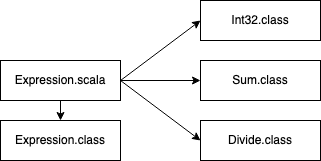
\includegraphics[scale=0.6]{img/Expression}
    \caption{Compilation result of Listing \ref{multidef}}
    \label{img:Expression}
\end{figure}

One might argue that multiple sizable class implementations with numerous methods contained in a singular source file are rare in actual code bases and optimizing for this case would yield minuscule benefits outside of tailored benchmarks, but the opposite is the truth. % todo: replace but a the opposite is true.
In the following example a typical usage of a popular Scala unit testing library Specs2 \cite{Specs2Github} is shown.

\lstinputlisting[language=Scala, linewidth=18cm, label={code:specs2code}, caption={Standard usage of Specs2}]{./specs2/SampleTest.scala}

Scala developers tend to use use many language features to create a Domain Specific Language (DSL) for visually pleasing code.
% TODO: maybe explain, but reword for sure
Because many Scala compiler feature are in play in this example, the details are quite intricate, but the result is that for each test case shown in the example \ref{code:specs2code} (first test, second test) a stand alone .class compilation output is created (SampleTest\$\$annon\$1.class, \$SampleTest\$\$anon\$2.class).
Having many unit tests in a sophisticated codebase can therefore increase the compilation times significantly, to a point where an iterative development process becomes impractical.
Compilation times longer than a minute can be easily surpassed when meticulously writing unit tests in a Test-driven development (TDD) approach.

%todo: reference to TDD book
TDD also promotes writing tests as a playground to explore approaches and test code feasibility before writing the implementation.
Long compilation times of unit tests make such an approach also impractical.

If an action takes more than 10 seconds the user is likely to loose attention and starts to perform different tasks \cite{Usability}.
The norm for compilers it to not show any kind of progress when compiling a single translation unit.
This exacerbates the perceived time it takes to complete a process for the user\cite{Usability}.

\subsection{Granularization}

As such the main idea of the thesis arises.
Instead of conceptually treating an entire file as single translation unit which needs to be recompiled in its entirety producing multiple output files, all the objects declared in a source file get treated as as distinct translation units.

It is a natural fit, every class declared in a the source already produces its own output, which is independent from other produced outputs.
Thanks to the language structure of modern programming languages, most of the top level constructs within the source files are classes.
Once a file has been loaded and parsed, all top level objects can be processed separately.
Separation enables the ability to process the translation units in parallel, the ability to skip already processed translation units. In other words, it enables us to granularize the giant translation unit into smaller translation units.
% todo: ka cia parasyti dar?

\section{Compiler}
% todo: the targeted optimizations - what optimizations?
At the start of the bachelor thesis a thorough investigation was made to analyze how the official Scala compiler works \cite{ScalaGithub} and if it is feasible to apply the targeted optimizations to it.
The investigation took very long and yielded little results, the codebase was too humongous and complicated to understand, the compiler too feature packed to adjust with the target objectives.
% todo: word it differently
% todo: pervedimas, i goalus nera konkretus, tiesiog pradedu tai daryti
Not being proficient enough in the codebase of the official Scala compiler and taking the scope of the bachelor thesis into account, it was deemed to complicated to undergo such a task.

Instead of adjusting an already existing compiler, a compiler was written from scratch with an iterative approach.
In the following numerous advantages and disadvantages of this method are expressed.

\textbf{Flexibility} - mature compilers are harder to change, they have accumulated a lot of code which needs to be adjusted for every modification.
The official Scala compiler has a complex pipeline with multiple passes and figuring out where what the best point of incision is a difficult task.
A small compiler written from scratch allows the author to focus on the most important aspects.

\textbf{Correctness} - ensuring that a new feature is correctly implemented in a sizable code base is an immense undertaking.
% todo: ensure is repeating/remove in order
In order to ensure that a new feature addition doesn't impact the overall behavior of the compiler every feature needs to be tested for correctness.
% todo: explain multi-pass and split sentence.
The multi-pass nature of the official Scala compiler makes reasoning about correctness difficult, because it is a non trivial undertaking to reason about how caching in one pass might affect functionality in subsequent passes.

\textbf{Simplicity and transparency} - a small compiler is simple and easy to reason about.
Writing one from scratch means that a complete understanding of the compiler exists.
New features are easier to add because of a complete understanding of the entire code base.
Debugging is much more pleasant since the number of affected features is smaller.

\textbf{Accuracy} - the results might be skewed since the self written compiler implements only a handful of features of the official language standard.
This can go both ways.

% todo: add references (
Some elaborate Scala features like type-driven implicits and mixing multiple traits are computationally very intensive.
The former needs to recurs in a nondeterministic way on distinct implicit types in order to find a correct type inheritance path while the latter creates a proxy method in a target classes for every method within a mixed in non trivial trait.
Being able to reuse computation instead of redoing these kind of workloads might add significant performance boosts.

On the other hand, adding a multitude of features might slow down general compilation speeds of the compiler.
Features that are not used should not add a significant slow down to execution speed, but code bases are rarely ideal.

\subsection{Language}
The target compiler programming language is Scala.
%Scala mixes multiple OOP and functional programming paradigms extensively creating a feature rich environment for developers.
%Functions in Scala are values and all values are objects which
Scala mixes object oriented programming (OOP)  and functional programming paradigms to create a feature rich environment for developers.
Functions in Scala are values and all values are objects, a smart way to seamlessly integrate both paradigms in a potent mix.

OOP has become quite ubiquitous and is a base line feature that most of programming languages have.
Many developers are proficient in at least one programming language supporting OOP and the most popular programming languages utilize OOP very prominently.

% https://data-flair.training/blogs/scala-features-comprehensive-guide/
The language aims to be concise and aesthetically pleasing utilizing features such as comprehensive type inference to minimize verbosity.
Functional aspects are prominently represented with a lightweight syntax for anonymous functions, higher order functions, currying, lazy evaluation, Algebraic Data Types (ADT), higher order functions, pattern matching.

% https://livebook.manning.com/book/scala-in-depth/chapter-10/3
% http://englishonlineclub.com/pdf/Scala%20in%20Depth%20[EnglishOnlineClub.com].pdf
%todo: maybe make this longer?
%\subsection{Runtime}
Scala is a programming language targeting the Java Virtual Machine (JVM).
Running on the JVM allows Scala easily to utilize existing Java code, which is a tremendous advantage because utilizing existing Java code opens access to a plethora of well maintained libraries targeting a wide range of needs.
The opposite however is not always true since Scala has a lot of features which can not be directly translated to JVM bytecode which is the underlying instruction set powering the JVM.

\subsection{Implementation}
Creating a compiler from scratch for a non trivial small language is already a significant task.
% todo: need citation?
Programming languages have become quite complex containing multiple paradigms.
Scala is also a language with a staggering amount of features that increases the overall complexity of a compiler.
Each language feature on its on might look simple and be easy to understand but putting another cog in an already complex machine can prove to be difficult.

Not only does Scala have a multitude of features but some of the features are quite complex like macros, implicit type conversion and summoning, pattern matching, higher kinded types and type lambdas allowing a user of the language to implement language constructs \cite{Scala2Union, ShapelessGithub} which are challenging to understand even for experienced Scala developers and more so difficult to implement.

%todo: talk a bit of how academic this compiler is

Instead of writing the entire compiler from scratch at once containing all features a more conservative approach is taken.
The approach starts out with the most simplistic compiler imaginable, compiling a bare minimum example of the target programming language, a simple "Hello World" program (listing \ref{code:helloworld}).

\lstinputlisting[language=Scala, linewidth=18cm, label={code:helloworld}, caption={"Hello World" in Scala}]{./code/HelloWorld.scala}

% Context resolution
Identifier resolution is also omitted in the minimal first implementation, the function identifier "println" definition is hard-coded in the compiler at first instead of creating an identifier resolution mechanism which would include all identifiers from Predef\$ in every compilation unit \cite{Predef}.
Afterwards every feature that is needed is for the thesis is implemented keeping the set of features concise while allowing to prove the thesis goal.
This allows us to deal with the complexity of Scala on a per demand basis, only features that are required are implemented incrementally to keep overall complexity down \cite{IncrementalCompiler}.

The compiler follows a classic compiler design with a frontend, the parser, an intermediate representation and the backend, code generation targeting the JVM and Java byte code.

\subsubsection{Frontend}

The frontend starts with a classical lexical analysis step.
The entire content of a file is loaded at once into memory to avoid dealing with continuous invocations of slow kernel file system application programming interface (API) calls.
Characters are grouped into tokens and a stream of tokens is produced with special meaning attached to each token in accordance with the Scala language specification \cite{ScalaSpec}.
Keywords of the language have special tokens to represent them and numbers and identifiers generic ones.

This is followed by a parser which transforms the sequence of tokens into an abstract syntax tree (AST).
The chosen approach is heavily inspired by a functional programming approach called "Monadic Parsing" \cite{MonadicParsing}.

% todo: mention how easy it is to combine
Monadic parsing is a parsing approach where monadic properties of data structures are being heavily utilized to create a parsing mechanism that has a rather simple and concise data structure it operates on, the parser.
A parser is a transformation of a token stream to a list of results, with each result containing the parser product and a tail token stream.

Simple parsers can be easily defined on their own (listing. \ref{code:SimpleParser})

% https://tex.stackexchange.com/questions/35155/lstlisting-in-two-columns

\noindent
\begin{minipage}{.45\textwidth}
  \lstinputlisting[language=Scala, linewidth=7cm, label={code:SimpleParser}, caption={Parsing a token}]{./code/Number.scala}
\end{minipage}\hfill
\begin{minipage}{.45\textwidth}
  \lstinputlisting[language=Scala, linewidth=10cm, label={code:ComplexParser}, caption={Parsing an import}]{./code/Import.scala}
\end{minipage}

Complex parsers can be easily created by combining simple parsers (listing. \ref{code:ComplexParser}).
Utilizing monad composition and Scala's for comprehension the solution is terse and compact.
A classic functional programming approach to deal with complexity also widely known as a bottom-up approach.

Scala's functional programming community is thriving and many libraries exist which can be used to aid in the handling of monads.
% todo: scalaz book citation
Scalaz \cite{scalaz} was used in the implementation of the parser, it had the most candid interface for mondas to implement.

%Scala
%  - has a very nice functional programming community, wich provides a lot of functional programming libraries like cats, scalaz with support for mondas
% scala is mentioned here https://en.wikipedia.org/wiki/API

%todo: questionable if I have one
%\subsubsection{Intermediate representation}

%The intermediate representation (IR) is uncomplicated and easy to follow.
%It represents the language structure in a straight forward way just using case classes and sealed traits emulating using ADT.

%\lstinputlisting[language=Scala, linewidth=16cm, label={multidef}, caption={Intermediate Representation}]{./code/IR.scala}

\subsubsection{Backend}

The compiler targets the JVM just like the official Scala compiler and therefore the output of the backed are instructions for the JVM called Java bytecode.

Compared to other computer architectures the Java bytecode is a fairly high level representation mirroring the functionality of Java closely.
As such it has a an explicit notion of classes and groups functionality of classes in a singular file ‒ the class file \cite{ClassFileFormat}.

Other machine architectures such as x86-64, ARM and Sparc do not have a notion of classes with fields and methods or references to other classes.
Compilers directly compiling to these kind of architectures need to map their high-level language constructs to a much more simplistic instruction set, which has only a concept of registers and a linear memory model.
This requires a lot of additional that a compiler should do, but in our case the JVM takes care of a lot of this functionality when JITing.

The backend translates the frontend generated AST to an intermediate representation (IR) which is closely modeled after the class file format.
Afterwards it serializes the IR to the class file format, which can be executed by the JVM.

The class file format is split into a body and header part.
The header parts contains integer, string constants, method and field references.
The body part contains the structure of the class.
In order to save bytes and to avoid repeating constant definitions, the body references values in the header.

This makes the body depended and makes patching of the file hard.
Adding an additional constant in the header means the the entire body needs to be shifted, which is an expensive operation.
The main value in the IR is to avoid this split and encode all the constants directly in the IR structure, making each sub expression of the IR self contained and easily transferable.

Class files are designed to be standalone and independent.
All the information needed is contained in the class.
References to other methods and fields from other classes are a fully qualified identifiers.
This property is key for translation unit granularization.
% todo do I need to mention IR?

\subsection{Translation unit memoization}
%The main improvement proposed in this paper is to just not do work when you don't need to absolutely do it.
%The second best way to increase performance is to make the code
%The best way to increase performance is to usually avoid work.

Computers have a limited amount of resources available, mainly the CPU and RAM get utilized when running programs like compilers.
The execution of speed gets determined by how many instructions the application needs to execute in order fulfill its goal.
%todo: mauybe quote SIMD?
The execution speed of instructions is also variable, as some instructions can be executed faster or accept more data to be processed at once.

Programming language abstractions add more instructions to the final executable that need to be executed.
One way to optimize for performance is to remove these abstractions and use lower level abstractions, which are closer to the machine.
Achieve the same goal with less.%, however this requires careful crafting of code.

Another way is to completely avoid the execution of instructions, reuse work that was already done.
Do not work if it the work has already done.
This solution is used in the compiler on all top level AST object within a source file.

Before translating the AST, a cache is queried with the list of all hash codes of already compiled AST objects.
If the object already exists, no work needs to be done, otherwise the compiler pipeline is invoked as usual.
Once the compiler has finished, the cache is replaced with all the new hashes.

\section{Benchmarks}
In order to measure the efficiency of the proposed granularization technique, multiple measurements have been taken.
Measurements were taken of the prototype compiler with and without caching of the translation units enabled and then also a measurement was taken of the official Scala compiler on the same input.

In order to measure the time difference between a cached compilation and a full compilation the cache file containing the hash codes of the already compiled translation units is simply deleted triggering a complete run of the compiler on the next invocation.

% todo: gal visdelto istrinam
%The additional translation unit caching logic generates such a low overhead, that it was decided to just leave it during both runs to simplify measurements.
%The warming up of the JVMs JIT mechanism and the JVMs Garbage Collection (GC) mechanism times incur a higher cost and therefore the additional overhead is negligible.

In short the sequence during benchmark looked like this:

\begin{enumerate}
\item{Delete the cache}
\item{Run the prototype compiler, which generates the cache}
\item{Run the prototype compiler, which utilizes the cache of the previous run}
\item{Run the official Scala compiler}
\end{enumerate}

\subsection{Measurements}

%todo: what is a general time measurement?
During the compilation runs a general time measurement was taken measuring the entire time it took the compiler from start to finish, labeled "full" in the following.
Additional measurements were taken of the prototype compiler of the following compilation steps:

%todo: add reference to the table
\begin{enumerate}
\item{read - reading the source file}
\item{lex - lexing the input into lexemes}
\item{parse - parsing the stream of tokens into an ast}
\item{ast - the transformation step which converts the ast into a high level class file representation}
\item{class - serializing the higher level class file representation into the binary class file format}
\item{write - writing the serialized class file from memory files}
\end{enumerate}

These measurements were taken only for the prototype compiler.
The official compiler has a much more complex compilation pipeline consisting of more than 12 steps instead of singular ast step in the prototype compiler.
Its architecture is also noticeably different, utilizing the same caching technique might not be easy to apply at the same layers.
The additional metrics would add little value and would make the benchmarking results harder to read without actually implementing the caching mechanism on in the official compiler.

\subsection{Hard to measure metrics}
% todo: of the entire application
Combining all single compilation pipeline step measurements of the prototype compiler does not add up to the single measurement metric "full" of the entire application.
This is caused by the JVM JIT startup costs and and variable GC interruption time.
The JVM needs to load the jars, the class files of a jar, run in interpreted mode and then JIT the class files into executable assembly code.
Also the GC can happen unpredictably at any moment between measurements which can add.

When analyzing the collected metrics one should keep in mind the additional overhead that the JVM can have.

\subsection{Input variance}
In order to measure variance in code complexity, variable input had to be created.
The dimensions of the created classes were twofold:

\begin{enumerate}
\item{Classes - the number of classes a source file contains}
\item{Methods - the number methods each classes has}
\end{enumerate}

The generated input files have the following format:

\lstinputlisting[language=Scala, linewidth=18cm, label={code:generated}, caption={Generated source inputs}]{./code/Generated.scala}

The number of translation units within a source file is controlled by the number of classes.
The complexity of each translation unit is controlled by the number of methods each class contains.
%todo: reikia parasyti apie v

The methods are kept very simple, singular expressions containing a basic function call.
Even with trivial methods which do not take much computation to compile down a significant uplift in performance is achieved, presented in the later subsection.

To simulate various workloads different inputs where chosen ranging from 1 class to 100 in an input source file and from 0 to 100 methods.

\subsection{Discussion}

Improvements from 20ms to 480ms can be observed during recompilation (figure \ref{graph:speed}).
This corresponds to an increase of 5\% and 30\% when considering the total run time of the compiler (figure \ref{graph:speed_pct}).

20ms is a value so small that it is hard to notice for the user of a compiler.
However, shaving off 322ms in a complex translation unit with 50 classes and 50 methods when the entire compilation takes 1084ms (table \ref{tb:benchmarks}) is significant and actually noticeable to the user of the software.

Applying the approach results in a performance increase of 5\% in the most trivial cases with no downside.
When a source file is very complex containing 100 translation units with each translation unit also being very complex containing 100 methods an improvement of up to 30\% can be observed.

In general an improvement in performance from 5\% to 15\% should be expected in normal scenarios.
In a scenario where a lot of code generation is involved an improvement of up to 30\% can be expected.


\begin{figure}
\caption{Speedup with caching}
\label{graph:speed}
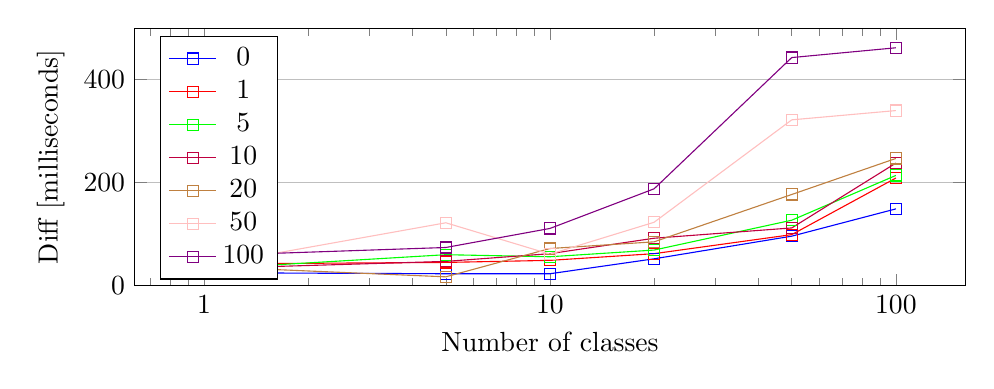
\begin{tikzpicture}
	\begin{axis}[
		ylabel={Diff [milliseconds]},
		width=1\textwidth, height=0.4\textwidth,
		ymin=0, ymax=500,
		xlabel={Number of classes},
		xmode=log,
		legend pos=north west,
		ymajorgrids=true,
		log ticks with fixed point,
	]

	%\addlegendentry{\hspace{-.6cm}\textbf{methods}}
	%addlegendentry{0}
	\legend{0, 1, 5, 10, 20, 50, 100}
	
\addplot[color=blue, mark=square]
  table {
       1   25
       5   23
      10   23
      20   52
      50   96
     100  149
  };

\addplot[color=red, mark=square]
  table {
       1   42
       5   45
      10   49
      20   62
      50   99
     100  209
  };

\addplot[color=green, mark=square]
  table {
       1   32
       5   60
      10   56
      20   69
      50  127
     100  214
  };

\addplot[color=purple, mark=square]
  table {
       1   33
       5   47
      10   62
      20   92
      50  112
     100  238
  };

\addplot[color=brown, mark=square]
  table {
       1   37
       5   17
      10   72
      20   85
      50  177
     100  247
  };

\addplot[color=pink, mark=square]
  table {
       1   38
       5  122
      10   61
      20  123
      50  322
     100  340
  };

\addplot[color=violet, mark=square]
  table {
       1   58
       5   74
      10  111
      20  188
      50  443
     100  462
  };


	\end{axis}
\end{tikzpicture}
\end{figure}

\begin{figure}
\caption{Speedup in percent}
\label{graph:speed_pct}
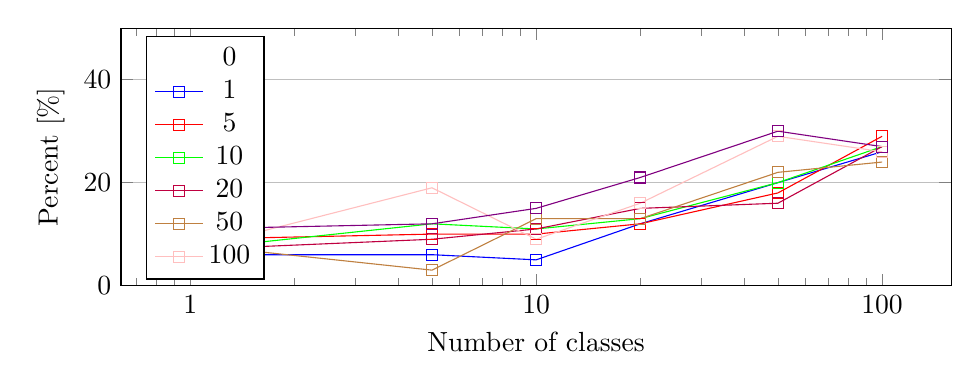
\begin{tikzpicture}
	\begin{axis}[
		ylabel={Percent [\%]},
		width=1\textwidth, height=0.4\textwidth,
		ymin=0, ymax=50,
		xlabel={Number of classes},
		xmode=log,
		legend pos=north west,
		ymajorgrids=true,
		log ticks with fixed point,
	]

	
\addlegendimage{empty legend}

\addplot[color=blue, mark=square]
  table {
       1    6
       5    6
      10    5
      20   12
      50   20
     100   26
  };

\addplot[color=red, mark=square]
  table {
       1    9
       5   10
      10   10
      20   12
      50   18
     100   29
  };

\addplot[color=green, mark=square]
  table {
       1    7
       5   12
      10   11
      20   13
      50   20
     100   27
  };

\addplot[color=purple, mark=square]
  table {
       1    7
       5    9
      10   11
      20   15
      50   16
     100   27
  };

\addplot[color=brown, mark=square]
  table {
       1    8
       5    3
      10   13
      20   13
      50   22
     100   24
  };

\addplot[color=pink, mark=square]
  table {
       1    7
       5   19
      10    9
      20   16
      50   29
     100   26
  };

\addplot[color=violet, mark=square]
  table {
       1   11
       5   12
      10   15
      20   21
      50   30
     100   27
  };


	\legend{0, 1, 5, 10, 20, 50, 100}

	\end{axis}
  \label{graph:speedup}
\end{tikzpicture}
\end{figure}

% Rezultatų skyriuje išdėstomi pagrindiniai darbo rezultatai: kažkas išanalizuota, kažkas sukurta, kažkas įdiegta. Rezultatai pateikiami sunumeruotų (gali būti hierarchiniai) sąrašų pavidalu. Darbo rezultatai turi atitikti darbo tikslą.
\sectionnonum{Results}

In this thesis the translation unit granularization concept has been presented.
An introduction was given to the current state of how compilers handle translation units in various programming languages.
An analysis was provided how the scope of a translation unit can be reduced by taking modern language features into consideration.

Scala was picked as a target language since it does not enforce a singular class per source file like Java.
The JVMs class file format also enforces a singular compilation output per class.
Singular Scala source files can therefore produce multiple compilation output files and therefore it is a natural fit for selective recompilation for changed output files.

It was pointed out that the size of the granularity of the translation units is directly related to compilation times.
To reduce compilation times in source code that does not change, granularization of big compilation units was proposed.

The official Scala compiler was deemed too complex and implemented in way which makes it too difficult for the author to adjust it to use the proposed approach.
For demonstration purposes of the viability of the presented approach, a prototype compiler has been written from scratch, implementing only a subset of the programming language, but designing it from the beginning with translation unit granularization in mind.

The prototype compiler was benchmarked with inputs of variable size and complexity.
To generate variable inputs a mechanism was presented and detailed, which creates inputs with a varying number of translation units and complexity for benchmark.
Various graphs were presented to better understand the performance improvements and the feasibility of the approach was discussed.

% Išvadų skyriuje daromi nagrinėtų problemų sprendimo metodų palyginimai, siūlomos rekomendacijos, akcentuojamos naujovės. Išvados pateikiamos sunumeruoto (gali būti hierarchinis) sąrašo pavidalu. Darbo išvados turi atitikti darbo tikslą.
\sectionnonum{Conclusion}

Translation unit granularization enables performance improvements by simply decomposing work units and then applying uncomplicated approaches to avoid redundant work.
%todo: reword
The smaller the translation unit is the less likely it is that a modification to the source code will result in a need redo work during recompilation.

Applying this approach to already existing compilers might prove to be difficult, but designing a compiler from the beginning with this approach in mind will lead to the possibly of easily increasing performance in the future.

When applying this methodology to a programming language as complicated as Scala, small benefits even to the inputs were measured to be at least 5\%.
The number of classes within a source file and the complexity of the classes have a noticeable effect on the performance increase.

A performance increase of up to 30\% was observed when the compiler needs to recompile the most complex source files.
This kind of complexity might only occur when a project utilizes a lot of code generation, for example, creating many objects from interface definition languages protocol buffers.

Compilation speed for code with complexity more often found in day to day development scenarios saw an improvement between 12\% and 16\%.

Applying translation unit granularization enables significant improvements to the recompilation speed and as such should always be considered when trying to improve the user experience of a compiler.

\iffalse
\sectionnonum{Future works}

Implementing unit granularization on a class level for source files was rather straight forward and showed very promising results.
The possibility of trying to further granularize the compilation units on a method level was met with a far greater challenges.

Method, field references and constants within a methods abstract syntax tree get encoded in the header of the class file.
The core structure of the abstract syntax tree gets encoded in the body.
However, the encoded structure within the body depends on the header because it refers with an offset number to constants described in the header.

Recompiling a singular method requires analyzing the target class file and patching the file accordingly.
The class file format is not really patch friendly.

If the newly compiled method body is bigger than the original in the class file, one might need to shift the rest of the file.
Introduction of constants in the header might also require the shift of the entire body part of the file.

Finer compilation unit granularization would require much more dedication to details, handling many corner cases, a lot of additional work and warrants a thesis on its own.
\fi

% (cituotų, perfrazuotų ar bent paminėtų) mokslo leidinių, kitokių publikacijų
% bibliografiniai aprašai. Šaltinių sąrašas spausdinamas iš naujo puslapio.
% Aprašai pateikiami netransliteruoti. Šaltinių sąraše negali būti tokių
% šaltinių, kurie nebuvo paminėti tekste. Šaltinių sąraše rekomenduojame
% necituoti savo kursinio darbo, nes tai nėra oficialus literatūros šaltinis.
% Jei tokių nuorodų reikia, pateikti jas tekste.

% \sectionnonum{Sąvokų apibrėžimai}
\sectionnonum{Acronyms}

\textbf{AST} - Abstract Syntax Tree

\textbf{JVM} - Java Virtual Machine

\textbf{JIT} - Just In Time

\textbf{DSL} - Domain Specific Language

\textbf{TDD} - Test Driven Development

\textbf{OOP} - Object Oriented Programming

\textbf{ADT} - Algebraic Data Type

\textbf{API} - Application Programming Interface

\textbf{IR} - Intermediate Representation

\textbf{JRE} - Java Runtime Environment

\appendix  % Priedai
% Prieduose gali būti pateikiama pagalbinė, ypač darbo autoriaus savarankiškai
% parengta, medžiaga. Savarankiški priedai gali būti pateikiami ir
% kompaktiniame diske. Priedai taip pat numeruojami ir vadinami. Darbo tekstas
% su priedais susiejamas nuorodomis.

% https://tex.stackexchange.com/questions/28422/table-reference
\begin{center}
	\begin{table}
	  \caption{Benchmarking results}
	  \label{tb:benchmarks}

    \begin{tabular}{ c | c || c || c | c | c || c | c | c | c | c | c }
      Classes & Methods & Prototyp & Cached & Diff & Official \\
   1 &   0 &   376 &   351 &    25 &  1721 \\
   1 &   1 &   426 &   384 &    42 &  1595 \\
   1 &   5 &   421 &   389 &    32 &  1681 \\
   1 &  10 &   430 &   397 &    33 &  1624 \\
   1 &  20 &   445 &   408 &    37 &  1693 \\
   1 &  50 &   476 &   438 &    38 &  1760 \\
   1 & 100 &   516 &   458 &    58 &  1901 \\
   5 &   0 &   375 &   352 &    23 &  1549 \\
   5 &   1 &   427 &   382 &    45 &  1636 \\
   5 &   5 &   473 &   413 &    60 &  1687 \\
   5 &  10 &   481 &   434 &    47 &  1804 \\
   5 &  20 &   511 &   494 &    17 &  1941 \\
   5 &  50 &   614 &   492 &   122 &  2364 \\
   5 & 100 &   616 &   542 &    74 &  3004 \\
  10 &   0 &   386 &   363 &    23 &  1616 \\
  10 &   1 &   448 &   399 &    49 &  1661 \\
  10 &   5 &   489 &   433 &    56 &  1863 \\
  10 &  10 &   537 &   475 &    62 &  2088 \\
  10 &  20 &   553 &   481 &    72 &  2335 \\
  10 &  50 &   621 &   560 &    61 &  2876 \\
  10 & 100 &   722 &   611 &   111 &  3794 \\
  20 &   0 &   413 &   361 &    52 &  1692 \\
  20 &   1 &   479 &   417 &    62 &  1792 \\
  20 &   5 &   530 &   461 &    69 &  2073 \\
  20 &  10 &   580 &   488 &    92 &  2371 \\
  20 &  20 &   616 &   531 &    85 &  2784 \\
  20 &  50 &   742 &   619 &   123 &  3688 \\
  20 & 100 &   894 &   706 &   188 &  4147 \\
  50 &   0 &   476 &   380 &    96 &  1883 \\
  50 &   1 &   541 &   442 &    99 &  2282 \\
  50 &   5 &   625 &   498 &   127 &  2676 \\
  50 &  10 &   675 &   563 &   112 &  3115 \\
  50 &  20 &   788 &   611 &   177 &  4140 \\
  50 &  50 &  1084 &   762 &   322 &  5111 \\
  50 & 100 &  1440 &   997 &   443 &  5452 \\

    \end{tabular}
  \end{table}
\end{center}

\printbibliography[heading=bibintoc]

\end{document}
